\chapter{Introduction}
\label{chpt:introduction}

The MCC inhibits the Anaphase-Promoting Complex/Cyclosome (APC/C) to delay anaphase onset (Izawa and Pines, 2015; Sudakin et al., 2001). This delay enables the unattached kinetochores to attach to spindle microtubules and thereby ensures accurate chromosome segregation.

% Unattached kinetochores catalyze MCC formation by recruiting SAC proteins in a well-defined signaling cascade (Fig. 1A) (Faesen et al., 2017; Ji et al., 2017; Lara-Gonzalez et al., 2021a; London and Biggins, 2014; London et al., 2012; Piano et al., 2021; Primorac et al., 2013; Shepperd et al., 2012). This cascade is activated when the kinetochore protein Knl1 is phosphorylated by the Mps1 kinase at the ‘MELT’ motifs, so called because of their consensus amino acid sequence in humans and other eukaryotes (Primorac et al., 2013; Tromer et al., 2015; Vleugel et al., 2013). Each MELT motif serves as the scaffold for recruiting downstream signaling proteins (Chen et al., 2019; Primorac et al., 2013).

%The parental HeLa-A12 cell line possesses an \GE{lox2272}-\GE{loxP} cassette for stable transfection \cite{HeLa-A12}. and offers great ease for automatic cell tracking during prolonged time-lapse imaging

% explain the core SAC signaling cascade vs RZZ pathway: An unattached kinetochore activates the SAC by allowing Mps1 kinase to phosphorylate KNL1 at sites known as MELT motifs due to their consensus sequence (Figures 1B and 1C) [7–10]. This event is followed by the sequential recruitment of Bub3-Bub1 and Mad1-Mad2, along with Bub3-BubR1 and Cdc20 to the kinetochore, with Mps1 phosphorylation playing a licensing role for each step (Figure 1B) [2, 11–19]. We refer to this biochemical cascade as the ‘‘core SAC signaling cascade’’ (dashed gray box in Figure 1B). In metazoa, the core SAC signaling cascade is complemented by the RZZ pathway, which independently recruits additional Mad1-Mad2 to the kinetochore [20]. Ultimately, Bub3, BubR1, Mad2, and Cdc20 form the MCC, which then disperses throughout the cellular volume to inhibit APC/C.

% Cooperativity

% Accurate chromosome segregation during cell division requires that the sister kinetochores on each replicated chromosome are stably attached to microtubules emanating from opposite spindle poles before the cell divides. If one or more kinetochores fail to attach to microtubules, they activate a biochemical signaling cascade known as the spindle assembly checkpoint (SAC). This cascade produces an anaphase-inhibitory signal known as the ‘‘mitotic checkpoint complex’’ (MCC). MCC in- hibits the anaphase promoting complex/cyclosome (APC/C) to prevent the cell from transitioning from prometaphase to anaphase, thus avoiding chromosome mis-segregation [2].

% The kinetochore-localized signaling activity of tightly clustered \protein{Knl1} molecules.

\begin{figure}
    \centering
    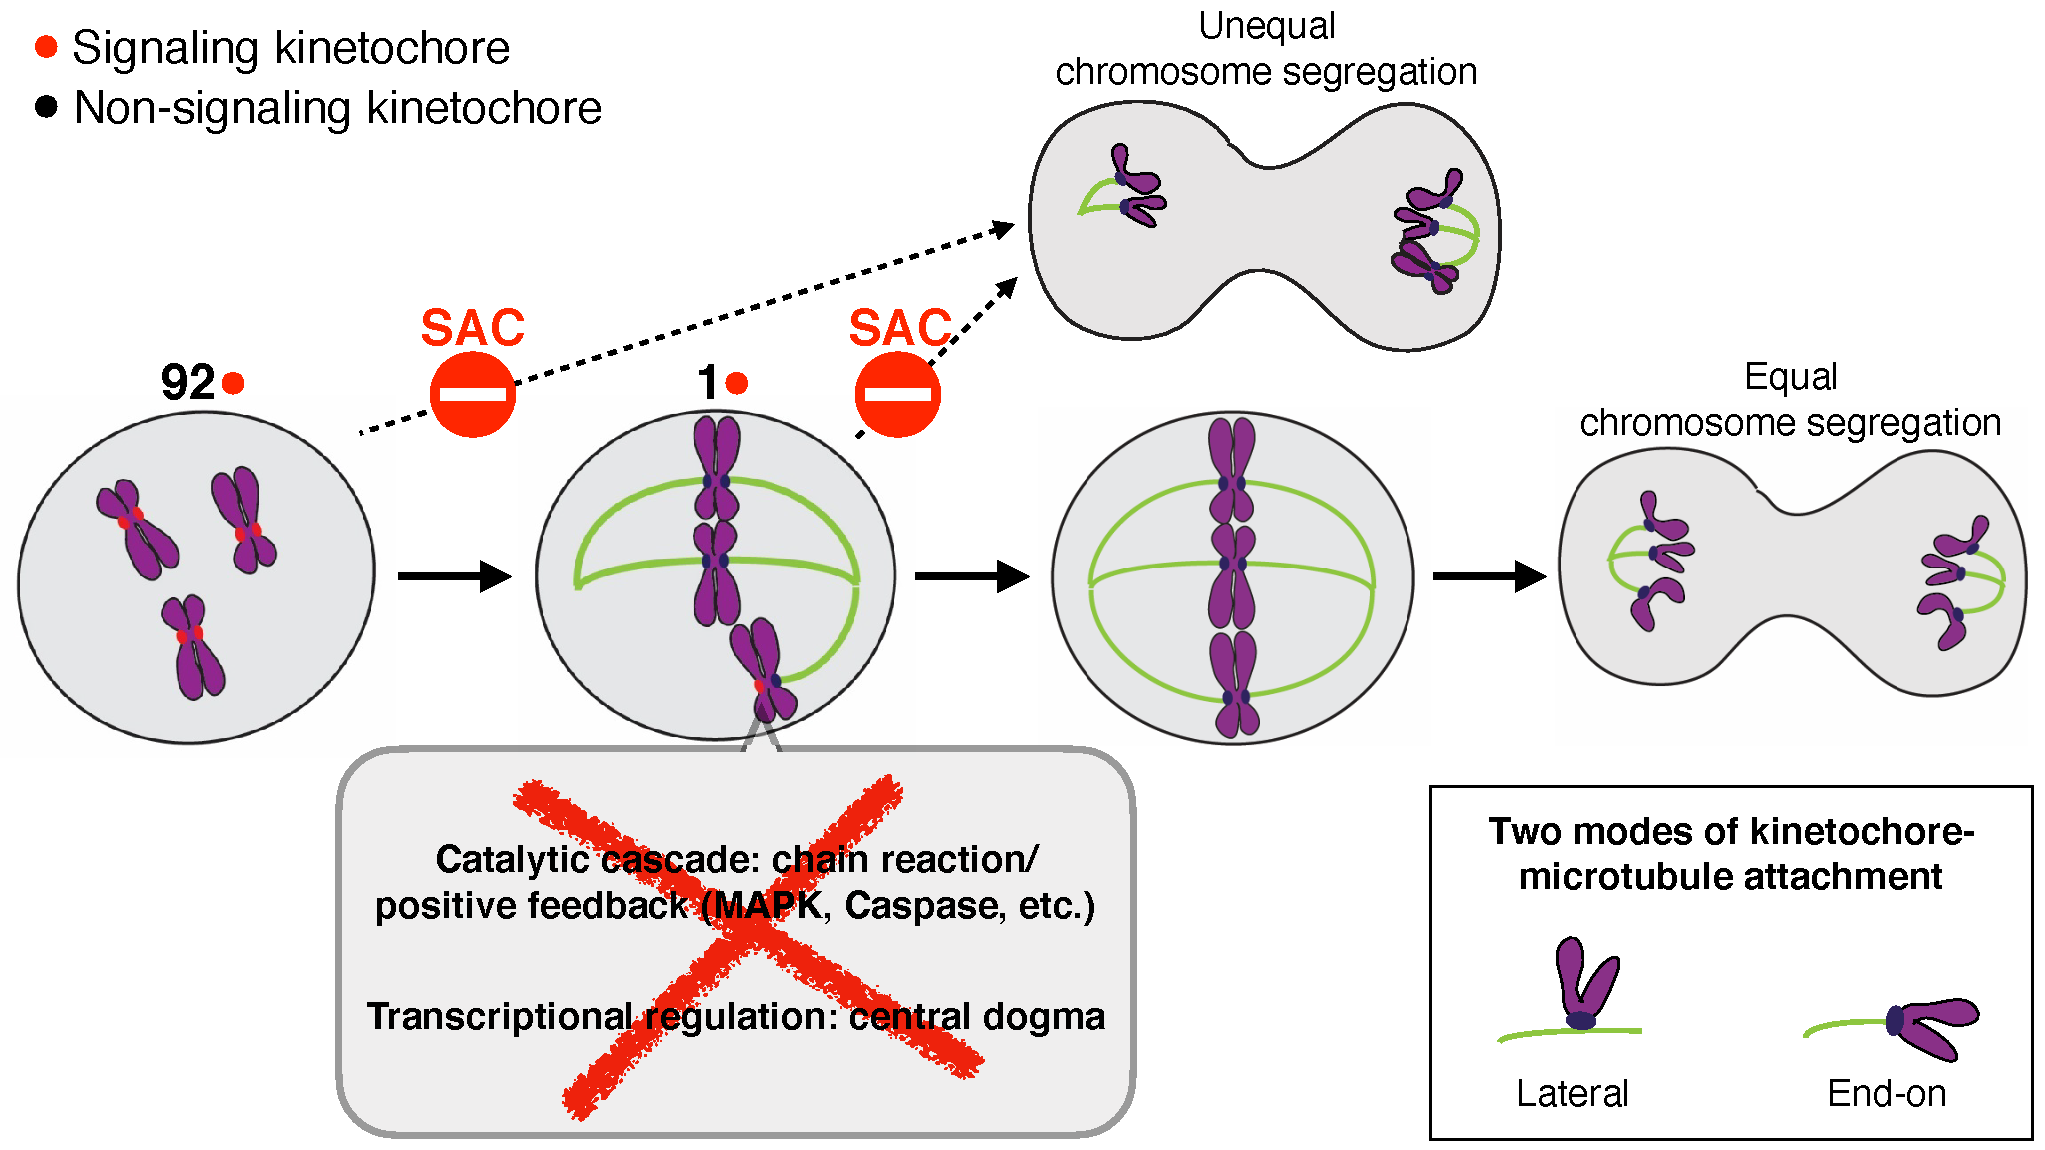
\includegraphics[width=0.95\textwidth]{chapters/figures/SACRole.pdf}
    \caption{\textbf{A diagram illustrating the role and properties of the spindle assembly checkpoint (SAC).}}
    \label{SACRole}
\end{figure}

% Figure: KNL1 19 putative MELT motifs & Biochemical event scheme of SAC

The spindle assembly checkpoint (SAC) is a signaling pathway in mitosis that delays anaphase onset in the presence of kinetochores lacking end-on attachment to spindle microtubules \cite{LateralAttachmentSAC}. The SAC can be activated by a single unattached kinetochore, but the strength of the signaling output (as commonly quantified by the duration from the nuclear envelope breakdown to the anaphase onset or mitotic slippage) increases with the number of signaling kinetochores in mammalian cells \cite{RiederNormalProgression,Rheostat,Ablation}. How the number of signaling kinetochores changes the strength of the signaling output is not fully understood. This knowledge will help us comprehend how the SAC prevents premature anaphase onset in the presence of a decreasing number of signaling kinetochores from the nuclear envelope breakdown to the metaphase during normal mitotic progression.

The SAC in mammalian cells relies on the kinetochore-localized signaling scaffold \protein{Knl1} as well as the corona, a crescent-shaped fibrous structure near kinetochores without end-on attachment to spindle microtubules \cite{GSK923295LateralAttachmentEM,CoronaActivatesSAC}. \protein{Knl1} possesses multiple MELT motifs \cite{MELTEvolution}, which are phosphorylated at unattached kinetochores and dephosphorylated at kinetochores with end-on attachment to spindle microtubules. Phosphorylated MELT motifs recruit SAC proteins like \protein{BubR1}, \protein{Bub1}, and \protein{Mad1}, promoting the formation of the mitotic checkpoint complex. The mitotic checkpoint complex inhibits the ubiquitin ligase anaphase promoting complex/cyclosome (APC/C), which ubiquinates the key mitosis regulator Cyclin B1 and targets it to proteasome-mediated degradation. In addition to the \protein{Knl1} pathway, the corona also recruits \protein{Mad1} and contributes to the spindle assembly checkpoint signaling output.

The \protein{Knl1} and the corona machinery also contribute to mitotic progression by facilitating chromosome congression. \protein{Knl1}-recruited \protein{BubR1} binds to the phosphatase \protein{PP2A-B56}, which stabilizes the kinetochore-microtubule attachment. The corona recruits the centromere-associated kinesin \protein{Cenp-E}, which promotes end-on attachment to spindle microtubules. This chromosome congression-promoting function complicates the quantitative study of the SAC signaling output in live cells.

To study the quantitative relationship between the strength of the SAC signaling and the number of signaling kinetochores/the amount of SAC proteins localized to signaling kinetochores, The SAC was then activated by treating the cells with either GSK923295 or a high dosage of nocodazole. GSK923295 inhibits the ATPase activity of \protein{Cenp-E}, thereby disrupting chromosome congression and yielding small numbers of chromosomes near spindle poles in mammalian cells \cite{GSK923295}.
% when applied at 75 nM -- 236 nM used in this study
These polar chromosomes typically possess one kinetochore that is unattached or laterally attached to spindle microtubules, both of which activate the SAC in mammalian cells \cite{GSK923295MonastrolCotreatment,GSK923295LateralAttachmentEM,LateralAttachmentSAC}.
% Monastrol co-treatment may have created the bias towards unattachment instead of lateral attachment.
Nocodazole affects the dynamics of microtubules and distorts spindles at \SI{330}{nM} in human cells \cite{TypeIIISpindle_330nMNoc, RPE1+Noc}, turning on SAC signaling at almost all kinetochores based on the recruitment of SAC proteins (see below). We applied various fluorescence microscopy and spectroscopy techniques to quantify SAC proteins and their influence on the SAC in live cells \cite{eSAC}. % Small numbers of signaling kinetochores and relative enrichment of SAC proteins on them.


Mammals seem to be prone to truncation in the arrangement of MELTs (the number of MELTs and the spacing between them). Alternative splicing is common in intrinsically disordered regions mediating protein-protein interactions \cite{DisorderedRegionsAlternativeSplicing}. In many mammals, all of Knl1's MELT motifs within a single exon [which is one of the longest internal exons in these mammals (\myref{ExonLength})] and are not alternatively spliced. The splicing machinery has to deploy specific mechanisms to splice long exons like this correctly \cite{InternalExon}.

\begin{table}[H]
    \renewcommand{\arraystretch}{2}
    \caption{\textbf{The length of the exon encoding all MELT motifs in some mammals and its ranking among all curated internal exons in human and mouse.}}
    \noindent\justifying Sequences of MELT motifs were referred from \cite{MELTEvolution}. We verified that all MELT motifs reside within a single exon in all listed mammals and all identified alternative splice variants contain this exon. Coordinates of exons (of mouse and human) in the Consensus CDS Database were accessed on May 21, 2020. Exons from coding sequences with either a ``Public'' or a ``Reviewed, update pending'' status were pooled. Various coding sequences may share a common exon, which is hence recorded more than once in the database. Therefore, redundant entries were detected and removed. Exons were then sorted by length and the ranking of the MELT motif-encoding exon was calculated. Because there is no data for untranslated regions in the database, only internal exons were included in the analysis. However, it should be noted that the maximum length of an exon is restricted by the length of the encoded protein, and \protein{KNL1} is a long protein of \SI{2342}{} amino acids (the canonical isoform).
    \label{ExonLength}
    \begin{center}
        \begin{tabular}{c c c}
            \hline
            Species & Exon length (bases) & Ranking among all curated internal exons\\
            \hline
            Human & 5001* & $99.973\%$\\
            Mouse & 4497 & $99.975\%$\\
            Rat & 3439 & N/A\\
            Cattle & 4020 & N/A\\
            Elephant & 4023 & N/A\\ % What kind of elephant?
            Giant panda & 4017 & N/A\\
            Dog & 3837 & N/A\\
            Bonobo & 3927 & N/A\\
            \hline
        \end{tabular}
    \end{center}
    \footnotesize{*According to UniProtKB, this exon is about 166 bases shorter in one non-canonical isoform. This exon still includes all 19 putative MELT motifs.}
\end{table}


Other constituents of the corona include \protein{Cenp-E} and \protein{Cenp-F}, which interact with \protein{BubR1} and \protein{Bub1}, respectively \cite{CENPELocalization-BUBR1, CENP-FLimitsStripping}.